% Chapter Template

\chapter{Implementació} % Main chapter title

\label{Chapter7} % Change X to a consecutive number; for referencing this chapter elsewhere, use \ref{ChapterX}

Un cop decidit com serà el sistema, és a dir, quins requisits, objectius i abast tindrà, i quin disseny s'aplicarà en ell, el següent es parla de la implementació per si mateixa. Les decisions preses anteriorment i explicades en capítols anteriors han marcat el que s'explicarà en aquest capítol. En primera instància es realitzarà un repàs per les tecnologies i eines utilitzades durant el desenvolupament de \textit{Wisebite}, i per acabar es seguirà pels detalls de la implementació del projecte.

%----------------------------------------------------------------------------------------
% SECTION 1
%----------------------------------------------------------------------------------------

\section{Tecnologies i eines utilitzades}

Durant el desenvolupament del projecte s'ha utilitzat tot tipus de tecnologies, és per això que s'ha decidit subdividir-ho en quatre conceptes. Començant pels llenguatges de programació, seguint per les bases de dades, mencionant les eines utilitzades i finalitzant amb les llibreries externes utilitzades.

\subsection{Llenguatge de programació}

\textbf{\large Java}\cite{java}\\
Com es va comentar anteriorment en la decisió de l'arquitectura, es va decidir construir una aplicació Android. Aquest sistema operatiu permet desenvolupar el \textit{backend} de les seves aplicacions natives en Java, C++ i Kotlin. Donat que el desenvolupador tenia més coneixement en desenvolupament d'aplicacions Android en Java, es va decidir utilitzar aquest llenguatge. A més a més, en ser el llenguatge de programació més utilitzat en el món des de ja fa anys, la comunitat d'usuaris és molt gran. En conseqüència, la probabilitat de trobar solucions a possibles problemes que es poden ocasionar és molt més alta que pas amb els altres dos llenguatges.
\\\\
\textbf{\large XML}\cite{xml}\\
El desenvolupament del \textit{frontend} en Android es realitza en llenguatge d'etiquetes, específicament XML. A diferència del \textit{backend}, en aquest cas no es tenia elecció dins del context de desenvolupament d'aplicacions natives.
\\\\
\textbf{\large \LaTeX}\cite{latex}\\
La realització de la memòria del projecte ha estat realitzada amb el llenguatge de software lliure anomenat \LaTeX. És un llenguatge que et permet realitzar documents pdf a través d'unes directives. L'esforç inicial d'aprendre aquest llenguatge es va contemplar en la planificació temporal del projecte, i tot i conèixer que seria d'un període més o menys considerable, es va contemplar l'esforç com útil en el projecte per la professionalitat i la robustesa que reflecteix el document.
\\\\
\begin{figure}[H]
\centering

\includegraphics[scale=0.20]{Figures/java.png}

\includegraphics[scale=0.15]{Figures/xml.png}
\hspace{0.8cm}

\includegraphics[scale=0.20]{Figures/latex.png}
\caption{Llenguatges de programació}
\end{figure}

\subsection{Bases de dades}

\textbf{\large Firebase}\cite{firebase}\\
Com s'ha comentat en capítols anteriors amb més detall, aquest projecte utilitza Firebase com a base de dades. Aquesta base de dades no relacional de tipus clau-valor ha aportat molts avantatges en el desenvolupament de l'aplicació donades les seves característiques, que anaven acord amb els objectius de \textit{Wisebite}.
\\\\
\textbf{\large SQLite}\cite{sqlite}\\
Al ser una plataforma Android, l'ús d'SQLite ve implícit en el desenvolupament del projecte. Aquesta base de dades actua com a memòria cau per així optimitzar l'obtenció de recursos durant la navegació per l'aplicació.
\\\\
\begin{figure}[H]
\centering

\includegraphics[scale=0.30]{Figures/firebase.png}

\includegraphics[scale=0.10]{Figures/sqlite.png}
\caption{Bases de dades}
\end{figure}

\subsection{Eines}

\textbf{\large Android Studio}\cite{androidstudio}\\
Google, com a propietari d'Android, recomana l'ús d'Android Studio per al desenvolupament de les seves aplicacions natives. A més a més, gràcies a la col·laboració de \textit{JetBrains}, aquest IDE disposa de moltes funcionalitats que faciliten l'ús del desenvolupador. Es pot nodrir d'un gran seguit de \textit{plugins} que permet fer-te el programa teu i desenvolupar amb més qualitat.
\\\\
\textbf{\large Genymotion}\cite{genymotion}\\
Durant el desenvolupament, les proves principals de l'aplicació s'han realitzat amb un terminal físic. Tot i així, per provar com funciona l'aplicació en diferents dispositius s'ha utilitzat Genymotion, un emulador al qual li pots afegir tot tipus de dispositiu Android, sigui mòbil o tauleta. Així s'ha pogut experimentar i provar com ha quedat el disseny de la interfície en plataformes diferents.
\\\\
\textbf{\large TeXstudio}\cite{texstudio}\\
Per al desenvolupament de la memòria s'ha utilizat el IDE de \LaTeX, anomenat TeXstudio. Aquest IDE et permet escriure en \LaTeX, de forma més agradable i ràpida gràcies principalment als seus \textit{shortcuts}. A més a més, pots alimentar aquest programa de plugins que et facilitaran més la redacció de la memòria, com per exemple un plugin de \textit{Softcatalà} que et permet tenir un corrector ortogràfic i gramatical de català durant l'escriptura del document final.
\\\\
\textbf{\large Git}\cite{git}\\
L'ús de Git durant el desenvolupament de \textit{Wisebite} ha estat vital per a la construcció del producte final. El poder de poder tenir un conjunt de versions del teu programa ha permès desenvolupar de forma més fàcil i sense por a provar coses noves i no trencar el codi anterior.
\\\\
\textbf{\large GitHub}\cite{github}\\
GitHub és considerat el gestor de repositoris remots més conegut del sector. Gràcies a les funcionalitats de les quals disposa, com poden ser les \textit{issues} o les \textit{pull requests}, han permès tenir un codi documentat i poder tenir un bon històric del desenvolupament del projecte. En apartats posteriors s'explicarà amb més detall com a funcionat el flux de treball amb l'ús de GitHub.
\\\\
\begin{figure}[H]
\centering

\includegraphics[scale=0.06]{Figures/androidstudio.png}

\includegraphics[scale=0.38]{Figures/genymotion.png}

\includegraphics[scale=0.18]{Figures/texstudio.png}
\hspace{0.1cm}

\includegraphics[scale=0.2]{Figures/git.png}
\hspace{0.2cm}

\includegraphics[scale=0.13]{Figures/github.png}
\caption{Eines}
\end{figure}

\subsection{Llibreries externes}

\textbf{\large Google Play Services}\cite{googleplayservices}\\
La majoria d'aplicacions Android utilitzen aquesta llibreria, ja que et permet accedir a totes les APIs disponibles de les quals disposa Google. En aquest projecte s'ha utilitzat només per això l'API d'autentificació, ja que el \textit{Log in} de l'aplicació es fa via Google.
\\\\
\textbf{\large FloatingActionButton}\cite{floatingactionbutton}\\
Durant el desenvolupament del projecte es va voler integrar un \textit{FloatingActionButton}, botó molt característic del \textit{Material Design}, però amb un menú integrat. Característica que no estava disponible en les llibreries natives d'Android. És per això que es va integrar aquesta llibreria externa de software lliure que ho permetia.
\\\\
\textbf{\large Picasso}\cite{picasso}\\
En les funcionalitats de gestió d'usuari, era necessària la interacció de les imatges amb l'aplicació. Concretament, es necessitava carregar les imatges des d'un URL. Es va estar investigant quina era la millor opció i es va acabar optant per Picasso. Una llibreria externa de software lliure que et permet carregar imatges via un URL de forma molt fàcil. Aquesta llibreria a més t'emmagatzema de forma automàtica la càrrega d'imatge a la memòria cau, fet que optimitza la plataforma i millora el flux de l'usuari amb aquesta.
\\\\
\textbf{\large MPAndroidChart}\cite{mpandroidchart}\\
Una de les funcionalitats de les quals disposa l'aplicació, i que s'ha esmentat anteriorment, és l'anàlisi de dades del restaurant. És per això que es va voler introduir un conjunt de gràfiques per visualitzar més fàcilment l'estat estadístic del restaurant. \textit{MPAndroidChart} és una llibreria de software lliure que et permet realitzar tot tipus de gràfiques, ja sigui un histograma, un gràfic de barres o circular i molts més.
\\\\
\textbf{\large Lombok}\cite{lombok}\\
Per optimitzar més el desenvolupament del projecte es va voler utilitzar la llibreria externa de software lliure anomenada Lombok, que et permet tenir codis més nets i més fàcils d'entendre. Per exemple, amb un simple @Getter a la capçalera d'una classe et permet tenir totes les funcions get dels atributs privats de la classe en qüestió.
\\\\
\begin{figure}[H]
\centering
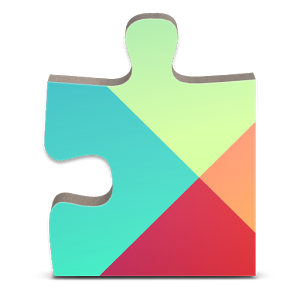
\includegraphics[scale=0.20]{Figures/googleplayservices.png}

\includegraphics[scale=0.20]{Figures/floatingactionbutton.png}

\includegraphics[scale=0.25]{Figures/square.png}

\includegraphics[scale=0.075]{Figures/mpandroidchart.png}

\includegraphics[scale=0.25]{Figures/lombok.png}
\caption{Llibreries externes}
\end{figure}

%----------------------------------------------------------------------------------------
%	SECTION 2
%----------------------------------------------------------------------------------------

\clearpage
\section{Detalls de la implementació}

Durant la implementació del projecte s'han seguit un conjunt de directrius específiques que han marcat l'estat final del producte. En aquest apartat s'explicarà en primera instància la metodologia d'implementació que s'ha seguit per obtenir un bon codi, i finalment com s'ha redactat la memòria amb l'ús, com s'ha comentat anteriorment, de \LaTeX.

\subsection{Implementació de l'aplicació}

La implementació de la qual disposa \textit{Wisebite} no conté cap algorisme de computació molt complex, més aviat són operacions trivials. És per això que s'ha volgut emfatitzar en com el codi ha anat evolucionant i com s'ha volgut remarcar la importància de tenir un codi ben documentat, ja que el codi sempre es llegirà més cops dels que s'escriurà. Per tant, es important tenir aquest aspecte en compte.
\\\\
Al seguir una metodologia àgil, com es va comentar en els primers capítols, és fàcil subdividir les tasques en històries d'usuari, les quals componen una funcionalitat independent del sistema. Així doncs, utilitzant les eines que ens facilita \textit{git} i \textit{GitHub}, es realitzava una branca per cada una de les històries d'usuari que s'implementava i cada \textit{bug} o error que es trobava. Entenem com a branca o \textit{branch} un mètode per ramificar part del codi d'un projecte, és a dir, desenvolupar part del codi de forma independent a la resta.
\\\\
Aquest concepte té molt sentit en treballs en equip, ja que molts membres poden treballar de forma independent tot i tocar codi del mateix projecte. Malgrat que aquest projecte sigui individual no impedeix que les branques deixin de ser útils. Permet veure, amb una mica de retrospectiva, l'evolució del codi i garantir que el codi publicat en la branca principal (coneguda com \textit{master}) és el correcte i funcional en plenes condicions.
\\
\begin{figure}[H]
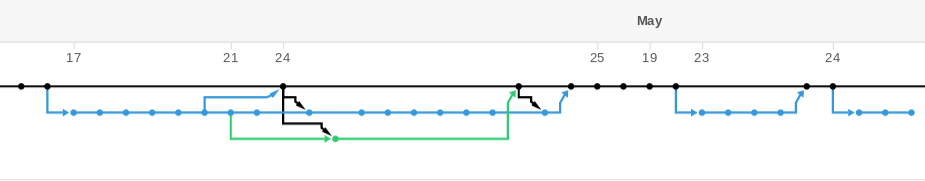
\includegraphics[scale=0.435]{Figures/branches.png}
\caption{Gestió de branques}
\end{figure}

\noindent Un cop el codi d'una branca estava finalitzat es creava una \textit{pull request} per revisar els canvis i acceptar-la en cas que fos correcte. Entenem \textit{pull request} com un conjunt de canvis que es volen revisar per ser acceptats i ser fusionats amb la branca principal. Al ser un treball individual la revisió només la realitza el desenvolupador del fragment de codi a revisar, però et permet disposar d'un historial de canvis i saber quina ha estat l'evolució i quan es van realitzar els canvis.
\\
\begin{figure}[H]
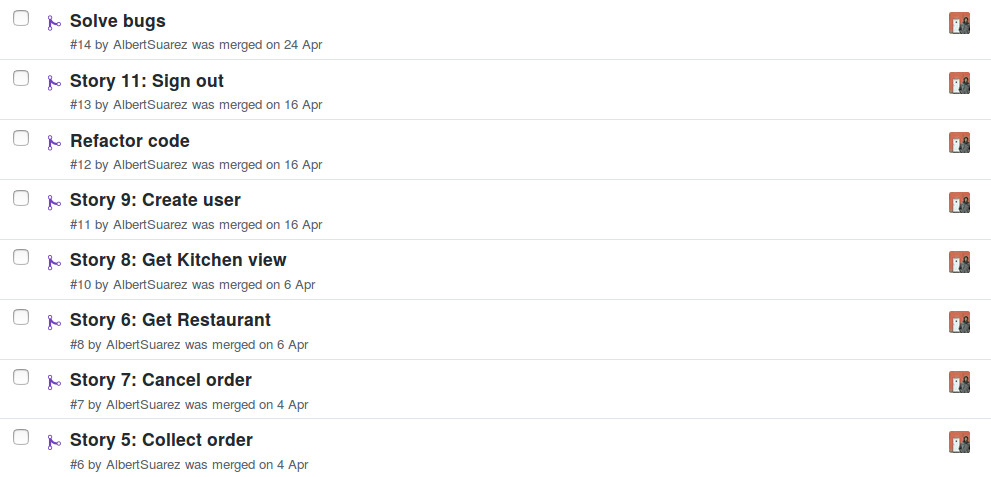
\includegraphics[scale=0.4]{Figures/pullrequests.png}
\caption{Gestió de pull requests}
\end{figure}

\noindent Així doncs el codi va evolucionant segons s'ha explicat, és a dir, mantenint la branca principal sempre funcional i desenvolupant en branques independents de la \textit{master}. Seguint aquesta metodologia es pot obtenir un codi prou documentat. Tot i així, com es pot arribar a entendre, hi ha punts dins la cronologia del codi que són més importants que la resta. Per aquest motiu s'ha decidit realitzar diferents versions del codi, les quals s'han anat provant amb usuaris externs al sistema, aspecte que es comentarà en el capítol següent.
\\\\
Per a poder posar a la pràctica aquest fet s'utilitzen els \textit{tags} o les \textit{releases} de GitHub. Aquestes eines et permeten marcar de manera destacada un punt de la cronologia del codi i posar-li un nom i una descripció. Així doncs, durant l'historial el codi de \textit{Wisebite} s'han indicat deu etiquetes amb les respectives versions del codi.
\\
\begin{figure}[H]
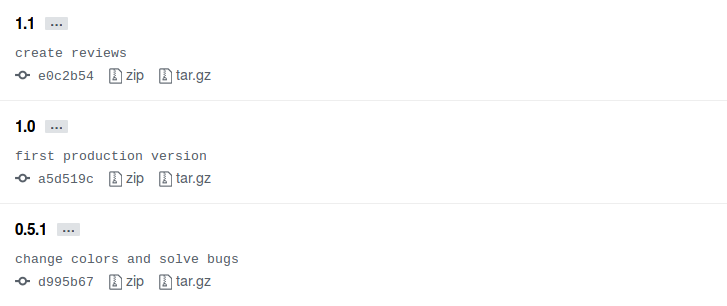
\includegraphics[scale=0.55]{Figures/tags.png}
\caption{Gestió de tags}
\end{figure}

\noindent Per altra banda també s'ha utilitzat les \textit{issues} de GitHub com un estil de bloc de notes amb els errors o millores que es volen realitzar a la plataforma i que en aquell moment no eren prioritats.
\\\\
I per últim, i ja lluny de la gestió de versions del codi i de la seva cronologia, s'ha utilitzat \textit{JavaDoc} com a estil de documentació del codi Java. Per així emfatitzar en el concepte que el codi es llegeix més cops del que s'escriu.

\subsection{Implementació de la memòria}

La metodologia que s'ha seguit per construir i redactar la memòria d'aquest treball final de grau consisteix en un conjunt de directrius.
\\\\
En primera instància es va dissenyar meticulosament el \textit{outline} de la memòria repassant la manquesa d'elements crucials que no havien de faltar. Perquè el marge d'error fos el menor possible el director del projecte va ajudar l'alumne facilitant-li exemples de memòries d'alumnes que ell va portar amb anterioritat perquè veies l'estil que ha de tenir una memòria. Així doncs, amb la combinació d'aquests dos aspectes es va dissenyar el \textit{outline} o índex complet.
\\\\
Com a següent pas de la cronologia de la memòria, es van buscar plantilles en format \LaTeX. Un cop es va trobar la plantilla adient al que es necessitava, es va adaptar al projecte en qüestió i es va començar a redactar. El mètode de redacció s'ha basat, semblant a la implementació del codi, en les \textit{issues} de GitHub. Cadascun dels apartats s'enregistrava en el repositori i se li atribuïa una etiqueta indicant si l'apartat s'havia de modificar o bé redactar d'un bon inici.
\\
\begin{figure}[H]
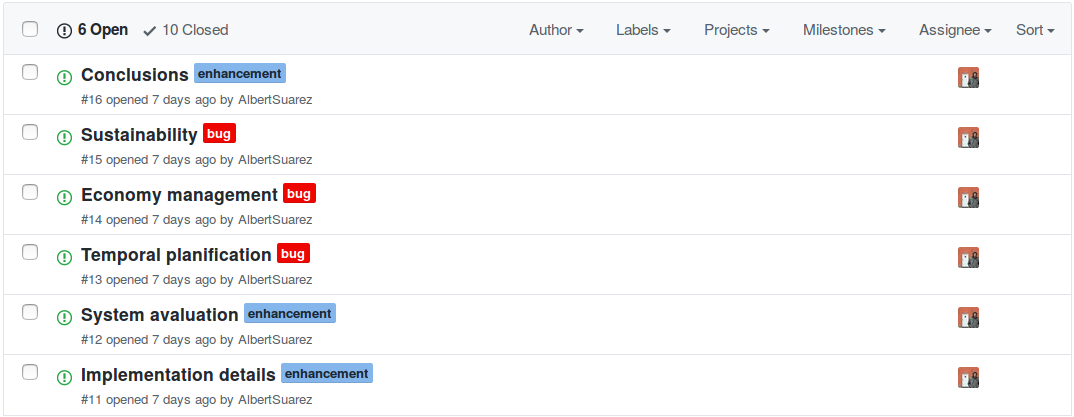
\includegraphics[scale=0.375]{Figures/issues.png}
\caption{Gestió d'issues}
\end{figure}

\noindent Les diferents versions de la memòria s'han anat validant per part del director del projecte, per així conèixer si el progrés d'aquesta és el correcte.